%% USPSC-Apendice.tex
% ---
% Inicia os apêndices
% ---

\begin{apendicesenv}
	% Imprime uma página indicando o início dos apêndices
	\partapendices
	\chapter{Additional tables of the textual differences found in all networks}\label{ap:textd}
In the following tables the counting of differences of textual features among the analyzed networks
are shown.
	These results are auxiliary for the discussion on Section~\ref{sec:tresults}.
\FloatBarrier
\begin{table}[h!]
\begin{center}
\caption{Counts of evidence of characters-related differences in the Erd\"os sectors in each of the analyzed networks.}
	\def\arraystretch{1.5}
\begin{tabular}{| l || c | c | c || c |}\hline
{\bf synset} & {\bf p.} & {\bf i.} & {\bf h} & {\bf peaks} \\\hline\hline
$\frac{spaces}{chars}$ & 2  & 0  & 8  & 2 \\
$\frac{punct}{chars-spaces}$ & 11  & 4  & 1  & 5 \\
$\frac{digits}{chars-spaces}$ & 9  & 7  & 2  & 10 \\\hline
$\frac{letters}{chars-spaces}$ & 0  & 0  & 3  & 0 \\
$\frac{vowels}{letters}$ & 0  & 1  & 1  & 1 \\
$\frac{uppercase}{letters}$ & 13  & 3  & 1  & 6 \\\hline
\end{tabular}
\begin{flushleft}
		Source: By the author.\
\end{flushleft}
\end{center}
\end{table}

\begin{table}[h!]
\begin{center}
\caption{Counts of evidence of token-related differences in the Erd\"os sectors in each of the analyzed networks.}
	\def\arraystretch{1.5}
\begin{tabular}{| l || c | c | c || c |}\hline
{\bf synset} & {\bf p.} & {\bf i.} & {\bf h} & {\bf peaks} \\\hline\hline
$\frac{knownw}{tokens}$ & 1  & 0  & 5  & 1 \\
$\frac{knownw \neq}{knownw}$ & 13  & 1  & 4  & 9 \\
$\frac{stopw}{knownw}$ & 0  & 0  & 14  & 2 \\
$\frac{punct}{tokens}$ & 10  & 3  & 1  & 3 \\
$\frac{contrac}{tokens}$ & 0  & 2  & 15  & 4 \\\hline
$\mu(\overline{tokens})$ & 0  & 1  & 2  & 1 \\
$\sigma(\overline{tokens})$ & 7  & 1  & 0  & 2 \\\hline
$\mu(\overline{knownw})$ & 0  & 0  & 2  & 0 \\
$\sigma(\overline{knownw})$ & 0  & 0  & 1  & 1 \\\hline
$\mu(\overline{knownw \neq})$ & 0  & 0  & 0  & 0 \\
$\sigma(\overline{knownw \neq})$ & 0  & 0  & 0  & 0 \\\hline
$\mu(\overline{stopw})$ & 0  & 0  & 0  & 0 \\
$\sigma(\overline{stopw})$ & 0  & 0  & 1  & 0 \\\hline
\end{tabular}
\begin{flushleft}
		Source: By the author.\
\end{flushleft}
\end{center}
\end{table}

\begin{table}[h!]
\begin{center}
\caption{Counts of evidence of sentence-related differences in the Erd\"os sectors in each of the analyzed networks.}
\begin{tabular}{| l || c | c | c || c |}\hline
{\bf synset} & {\bf p.} & {\bf i.} & {\bf h} & {\bf peaks} \\\hline\hline
$\mu_S(chars)$ & 9  & 3  & 1  & 6 \\
$\sigma_S(chars)$ & 11  & 6  & 1  & 9 \\\hline
$\mu_S(tokens)$ & 10  & 2  & 1  & 5 \\
$\sigma_S(tokens)$ & 9  & 7  & 1  & 9 \\\hline
$\mu_S(knownw)$ & 9  & 3  & 2  & 6 \\
$\sigma_S(knownw)$ & 11  & 5  & 2  & 8 \\\hline
$\mu_S(stopw)$ & 2  & 3  & 7  & 7 \\
$\sigma_S(stopw)$ & 6  & 7  & 4  & 10 \\\hline
$\mu_S(puncts)$ & 13  & 2  & 1  & 2 \\
$\sigma_S(puncts)$ & 7  & 8  & 1  & 8 \\\hline
\end{tabular}
\begin{flushleft}
		Source: Prepared by the authors.\
\end{flushleft}
\end{center}
\end{table}

\begin{table}[h!]
\begin{center}
\caption{Counts of evidence of message-related differences in the Erd\"os sectors in each of the analyzed networks.}
	\def\arraystretch{1.5}
\begin{tabular}{| l || c | c | c || c | c |}\hline
{\bf synset} & {\bf p.} & {\bf i.} & {\bf h} & {\bf peaks} & {\bf total} \\\hline\hline
$\mu_M(sents)$ & 4  & 7  & 1  & 9  & 16 \\
$\sigma_M(sents)$ & 5  & 7  & 2  & 11  & 15 \\\hline
$\mu_M(tokens)$ & 10  & 5  & 2  & 6  & 18 \\
$\sigma_M(tokens)$ & 8  & 8  & 2  & 9  & 18 \\\hline
$\mu_M(knownw)$ & 8  & 5  & 3  & 7  & 18 \\
$\sigma_M(knownw)$ & 10  & 5  & 3  & 9  & 18 \\\hline
$\mu_M(stopw)$ & 5  & 6  & 6  & 8  & 18 \\
$\sigma_M(stopw)$ & 7  & 6  & 3  & 11  & 18 \\\hline
$\mu_M(puncts)$ & 12  & 4  & 2  & 5  & 18 \\
$\sigma_M(puncts)$ & 8  & 9  & 1  & 10  & 18 \\\hline
$\mu_M(chars)$ & 10  & 5  & 2  & 6  & 18 \\
$\sigma_M(chars)$ & 9  & 7  & 2  & 8  & 18 \\\hline
\end{tabular}
\begin{flushleft}
		Source: Prepared by the authors.\
\end{flushleft}
\end{center}
\end{table}

\begin{table}[h!]
\begin{center}
\caption{Counts of evidence of differences related to POS tags in the Erd\"os sectors in each of the analyzed networks.}
\begin{tabular}{| l || c | c | c || c |}\hline
{\bf synset} & {\bf p.} & {\bf i.} & {\bf h} & {\bf peaks} \\\hline\hline
NOUN & 13  & 1  & 0  & 1 \\
X & 4  & 9  & 5  & 14 \\\hline
ADP & 0  & 1  & 4  & 1 \\
DET & 1  & 0  & 9  & 2 \\\hline
VERB & 0  & 0  & 6  & 1 \\\hline
ADJ & 1  & 2  & 6  & 2 \\
ADV & 0  & 0  & 17  & 1 \\\hline
PRT & 1  & 1  & 9  & 4 \\
PRON & 0  & 1  & 11  & 3 \\
NUM & 8  & 5  & 3  & 7 \\
CONJ & 2  & 6  & 4  & 8 \\\hline
\end{tabular}
\begin{flushleft}
		Source: By the author.\
\end{flushleft}
\end{center}
\end{table}

\begin{table}[h!]
\begin{center}
\caption{Counts of evidence of differences related to Wordnet POS tags in the Erd\"os sectors in each of the analyzed networks.}
\begin{tabular}{l || c | c | c || c}\hline
{\bf synset} & {\bf p.} & {\bf i.} & {\bf h} & {\bf peaks} \\\hline\hline
N & 8  & 1  & 0  & 1 \\
ADJ & 0  & 2  & 12  & 6 \\
VERB & 0  & 1  & 16  & 2 \\
ADV & 0  & 0  & 9  & 1 \\\hline\hline
POS & 0  & 0  & 3  & 1 \\
POS! & 0  & 1  & 0  & 1 \\\hline
\end{tabular}
\begin{flushleft}\footnotesize
		Source: By the author.\
\end{flushleft}
\end{center}
\end{table}

\begin{table}[h!]
\begin{center}
\caption{Counts of evidence of differences related to Wordnet noun synset characteristics in the Erd\"os sectors in each of the analyzed networks.}
\begin{tabular}{| l || c | c | c || c |}\hline
{\bf synset} & {\bf p.} & {\bf i.} & {\bf h} & {\bf peaks} \\\hline\hline
$\mu(min\,depth)$ & 0  & 0  & 0  & 0 \\
$\sigma(min\,depth)$ & 1  & 1  & 2  & 1 \\\hline
$\mu(max\,depth)$ & 0  & 0  & 0  & 0 \\
$\sigma(max\,depth)$ & 0  & 1  & 3  & 1 \\\hline
$\mu(holonyms)$ & 7  & 4  & 4  & 6 \\
$\sigma(holonyms)$ & 3  & 4  & 7  & 6 \\\hline
$\mu(meronyms)$ & 8  & 5  & 3  & 7 \\
$\sigma(meronyms)$ & 12  & 4  & 2  & 9 \\\hline
$\mu(domains)$ & 6  & 4  & 5  & 8 \\
$\sigma(domains)$ & 3  & 1  & 4  & 3 \\\hline
$\mu(lemmas)$ & 6  & 0  & 1  & 2 \\
$\sigma(lemmas)$ & 6  & 2  & 2  & 4 \\\hline
$\mu(hyponyms)$ & 1  & 6  & 6  & 9 \\
$\sigma(hyponyms)$ & 4  & 6  & 6  & 11 \\\hline
$\mu(hypernyms)$ & 0  & 0  & 0  & 0 \\
$\sigma(hypernyms)$ & 4  & 4  & 4  & 6 \\\hline
\end{tabular}
\begin{flushleft}
		Source: Prepared by the authors.\
\end{flushleft}
\end{center}
\end{table}

\begin{table}[h!]
\begin{center}
\caption{Counts of evidence of differences related to Wordnet adjective synset characteristics in the Erd\"os sectors in each of the analyzed networks.}
\begin{tabular}{| l || c | c | c || c |}\hline
{\bf synset} & {\bf p.} & {\bf i.} & {\bf h} & {\bf peaks} \\\hline\hline
$\mu(domains)$ & 2  & 6  & 8  & 10 \\
$\sigma(domains)$ & 2  & 4  & 5  & 7 \\\hline
$\mu(similar)$ & 1  & 0  & 7  & 4 \\
$\sigma(similar)$ & 4  & 0  & 5  & 3 \\\hline
$\mu(lemmas)$ & 1  & 2  & 1  & 2 \\
$\sigma(lemmas)$ & 6  & 3  & 4  & 6 \\\hline
\end{tabular}
\begin{flushleft}
		Source: By the author.\
\end{flushleft}
\end{center}
\end{table}

\begin{table}[h!]
\begin{center}
\caption{Counts of evidence of differences related to Wordnet verb synset characteristics in the Erd\"os sectors in each of the analyzed networks.}
\begin{tabular}{| l || c | c | c || c |}\hline
{\bf synset} & {\bf p.} & {\bf i.} & {\bf h} & {\bf peaks} \\\hline\hline
$\mu(min\,depth)$ & 2  & 1  & 1  & 3 \\
$\sigma(min\,depth)$ & 2  & 1  & 1  & 2 \\\hline
$\mu(max\,depth)$ & 2  & 1  & 0  & 1 \\
$\sigma(max\,depth)$ & 3  & 1  & 1  & 2 \\\hline
$\mu(domains)$ & 7  & 3  & 4  & 4 \\
$\sigma(domains)$ & 8  & 3  & 3  & 5 \\\hline
$\mu(verb\,groups)$ & 0  & 2  & 3  & 2 \\
$\sigma(verb\,groups)$ & 0  & 0  & 0  & 0 \\\hline
$\mu(lemmas)$ & 0  & 0  & 2  & 0 \\
$\sigma(lemmas)$ & 1  & 0  & 3  & 0 \\\hline
$\mu(entailments)$ & 7  & 1  & 7  & 3 \\
$\sigma(entailments)$ & 4  & 1  & 5  & 3 \\\hline
$\mu(hyponyms)$ & 1  & 2  & 6  & 3 \\
$\sigma(hyponyms)$ & 2  & 3  & 8  & 6 \\\hline
$\mu(hypernyms)$ & 2  & 2  & 0  & 2 \\
$\sigma(hypernyms)$ & 1  & 0  & 1  & 1 \\\hline
\end{tabular}
\begin{flushleft}
		Source: By the author.\
\end{flushleft}
\end{center}
\end{table}

\begin{table}[h!]
\begin{center}
\caption{Counts of evidence of differences related to Wordnet adverb synset characteristics in the Erd\"os sectors in each of the analyzed networks.}
\begin{tabular}{| l || c | c | c || c |}\hline
{\bf synset} & {\bf p.} & {\bf i.} & {\bf h} & {\bf peaks} \\\hline\hline
$\mu(domains)$ & 3  & 3  & 10  & 10 \\
$\sigma(domains)$ & 1  & 4  & 7  & 7 \\\hline
$\mu(lemmas)$ & 0  & 0  & 1  & 1 \\
$\sigma(lemmas)$ & 3  & 1  & 2  & 4 \\\hline
\end{tabular}
\begin{flushleft}
		Source: Prepared by the authors.\
\end{flushleft}
\end{center}
\end{table}


\chapter{Developments made in this research but not included elsewhere in this thesis}\label{ap:vot}
In this appendix are gathered developments relevant for the initial proposal of this research:
enabling the use of complex networks scientific knowledge by the participant of the social networks.
These developments are not included elsewhere in the thesis because we chose to present results
more closely related to physics in a simple fashion.
Furthermore, most of the following contributions have received dedicated documentation,
reason why we next only summarize and cite the documents when they are available.

\section{Continuous voting by approval and participation}
In finding the adequate way to prioritize proposals, the Brazilian social participation community agreed about the measurement of two indexes,
one of approval and one of participation. Both practice and literature
was constantly handled by the experts involved, and the formalization
of such model and metrics and is very simple and seems novel.
Also, the relevance of this development is strengthened by the use of these indexes by the
Brazilian General Secretariat of the Republic to raise and prioritize
proposals about public health care in open processes.
This was achieved by means of the Dialoga Brasil federal platform~\cite{dialoga}.
A short report on these indexes and their use is on~\cite{dialogaAlg}
	(co-authorship by Ricardo Poppi).

	\section{Visualization of static networks}
	In Sections~\ref{sec:versinus0} and~\ref{sec:versinus1} we addressed a visualization method of networks through animations.
	We also made many static network visualizations which were important for our research.
	Many of these were made by testing software and programming libraries.
	We next exemplify such efforts by probably the most important and time-consuming realizations.

	\subsection{Static email networks visualization using Networkx and Graphviz and a PHP web interface}\label{sec:autoRede}
	At the start of this research, we observed many networks derived from email lists
	by means of a web interface we wrote.
	In such web interface, which was accessed as a usual webpage through HTTP in a web browser, 
	the user could specify an email list, start and end messages and a window size (number of messages taken together to obtain the network).
	The interface then rendered graph visualizations and standard measures such as degree, strength, clustering coefficient, betweenness centrality, both as histograms and as mean and standard deviation.
	In the node-link diagrams, measurements were mapped to height, width and color of nodes and to link characteristics.
	The software source code is available in~\cite{autoRede} and an example image is Figure~\ref{fig:autoRede}.
\begin{figure}[h!]
\begin{center}
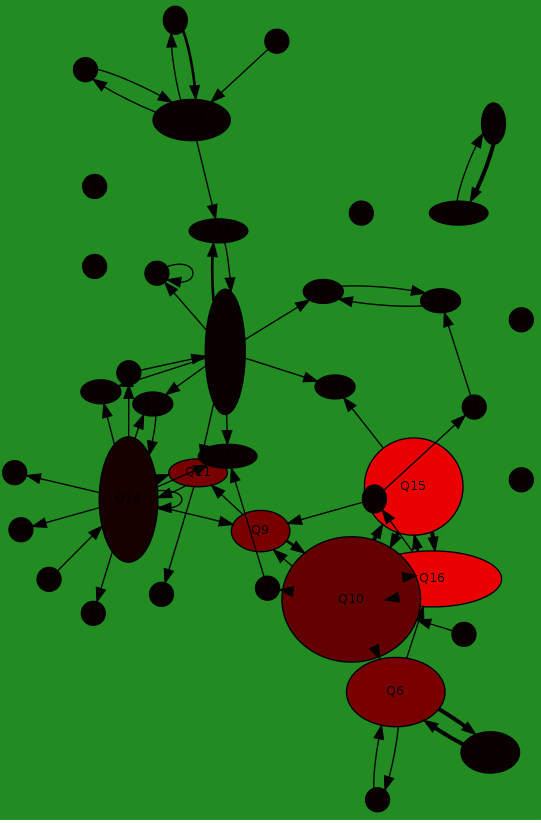
\includegraphics[scale=.25]{figs/autoRede_}
\caption{An example image rendered from the first online gadget made in this research for studying social networks.
	The app also delivered measurements, 2D plots and GML graph files. For further information please see Section~\ref{sec:autoRede}}
\label{fig:autoRede}
\begin{flushleft}\footnotesize
Source: By the author.\
\end{flushleft}
\end{center}
\end{figure}
% email pelo app online

	\subsection{Static Facebook networks visualization using Gephi}\label{sec:gephi}
	Mainly in the years of 2013 and 2014, Facebook users retrieved their friendship networks through Netvizz software~\cite{netvizz}
	and donated them to our research.
	I also retrieved friendship and interaction networks from Facebook groups I was a member, also using Netvizz.
	These networks were used for information collection and diffusion (explained in Section~\ref{sec:colDif}),
	taking measurements and visualization.
	The visualizations were achieved almost exclusively through the Gephi software~\cite{gephi}
	and is included in this appendix for being used a number of times by fellow researchers and artists.
	The most useful layout algorithm was Force Atlas 2~\cite{fa2} and an example of these images is Figure~\ref{fig:gephi}.

% \begin{figure}[h!]
% \begin{center}
% 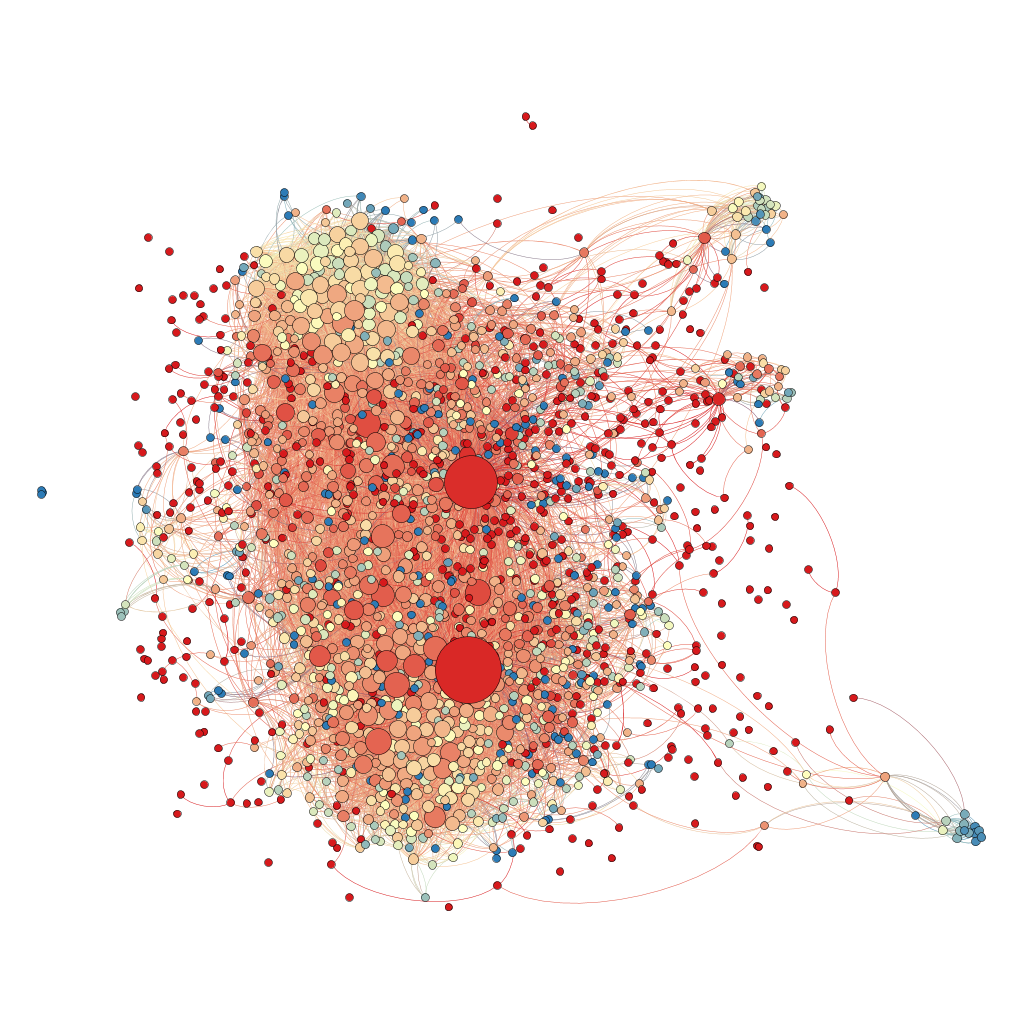
\includegraphics[scale=.25]{figs/Silicon}
% 	\caption{An example network image rendered from the Silicon Valley (Facebook) group using Gephi and the Force Atlas 2 layout algorithm.
% 	See Section~\ref{sec:gephi} for further information.}
% \label{fig:gephi}
% \begin{flushleft}\footnotesize
% Source: By the author.\
% \end{flushleft}
% \end{center}
% \end{figure}

\begin{figure}[!tbp]
	\centering
	    \subfloat[\footnotesize Without participant names.]{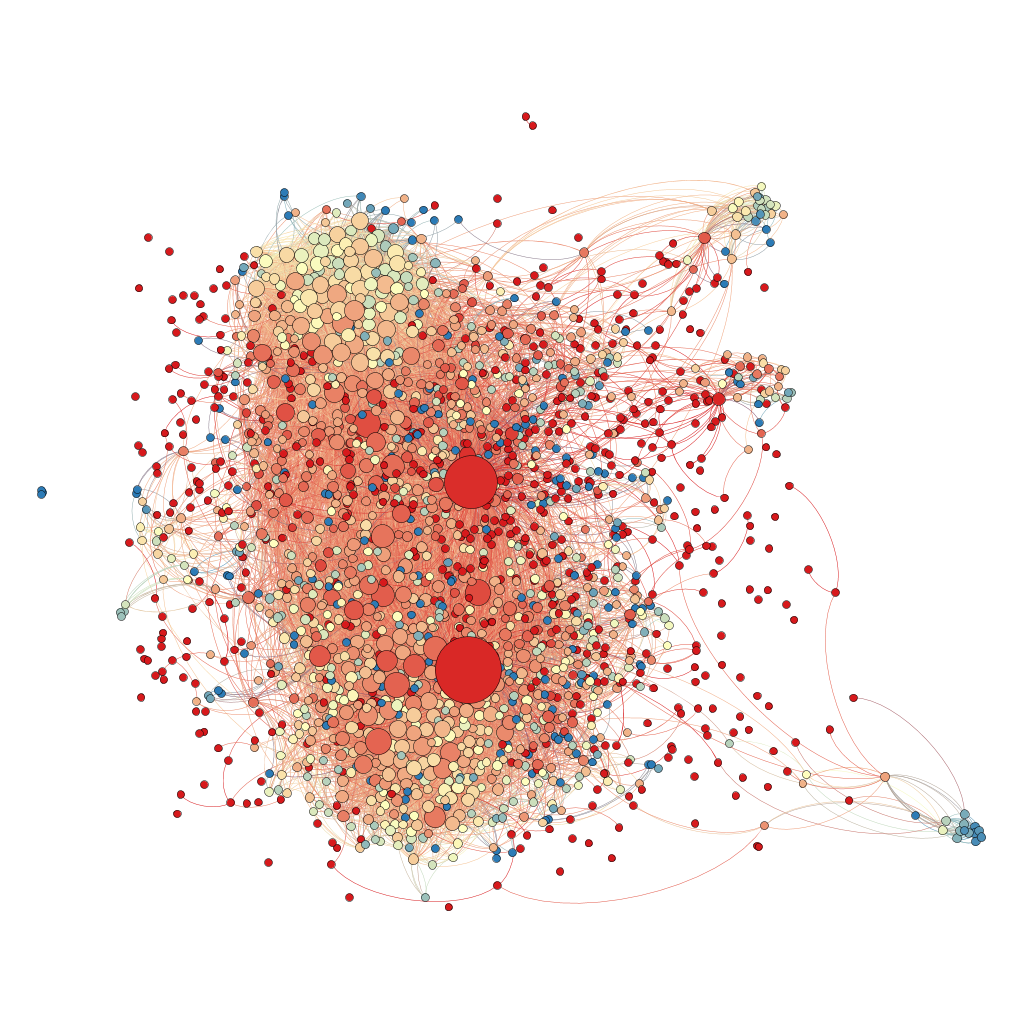
\includegraphics[width=0.45\textwidth]{figs/Silicon.png}\label{fig:f1}}
		\subfloat[\footnotesize With participant names.]{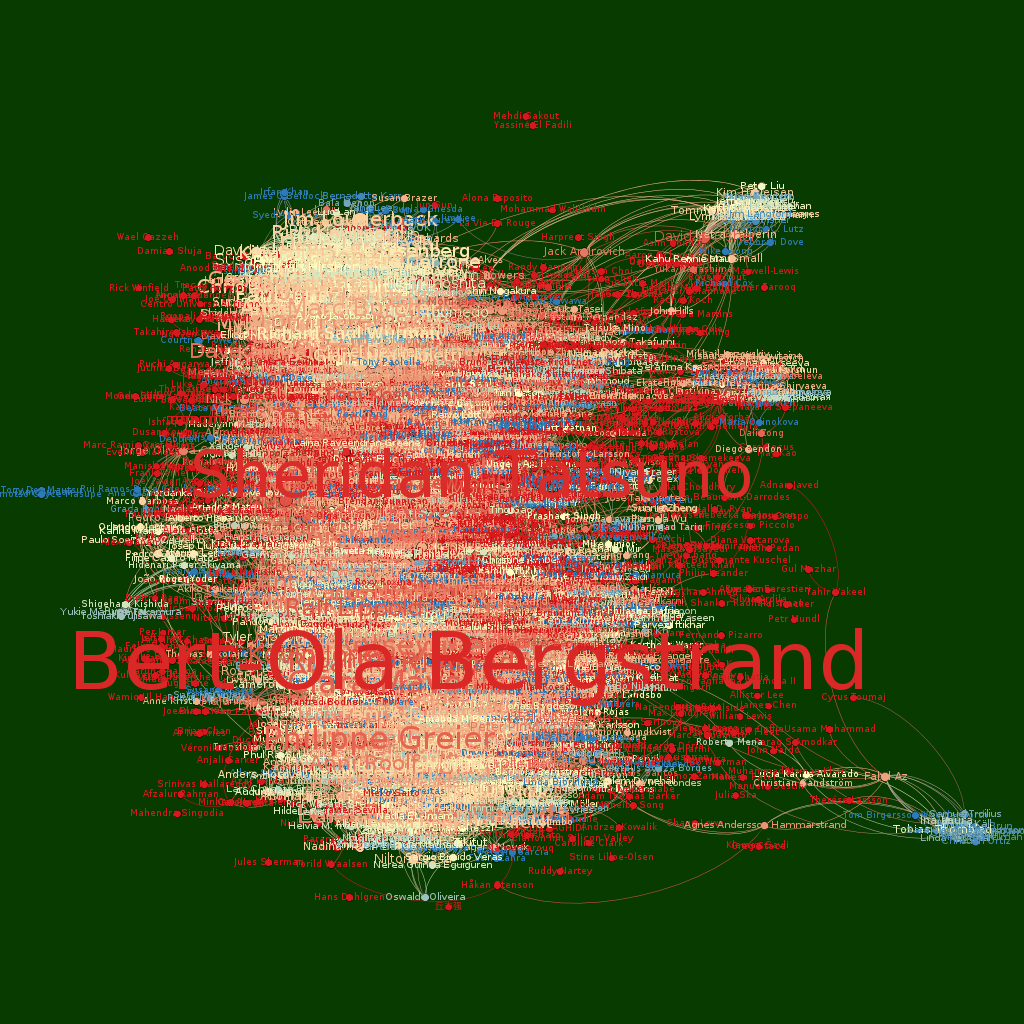
\includegraphics[width=0.45\textwidth]{figs/Silicon_nomes.png}\label{fig:f2}}
	\caption{An example network image rendered from the Silicon Valley (Facebook) group using Gephi and the Force Atlas 2 layout algorithm.
	See Section~\ref{sec:gephi} for further information.}\label{fig:gephi}
\begin{flushleft}\footnotesize
Source: By the author.\
\end{flushleft}
\end{figure}

	\subsection{Art by Pedro Paulo Rocha}\label{sec:ppr}
	The static images rendered for the visualization of networks were at time also used for artistic elaborations.
	Apart from other artistic incidences reported in this appendix (such as in Sections~\ref{sec:govArt} and~\ref{sec:soundSkull})
	we present in Figure~\ref{fig:ppr} an example art from Pedro Paulo Rocha.
	More of his work that is derived from our network visualizations are gathered in an image Gallery~\cite{pprGal}.
\begin{figure}[h!]
\begin{center}
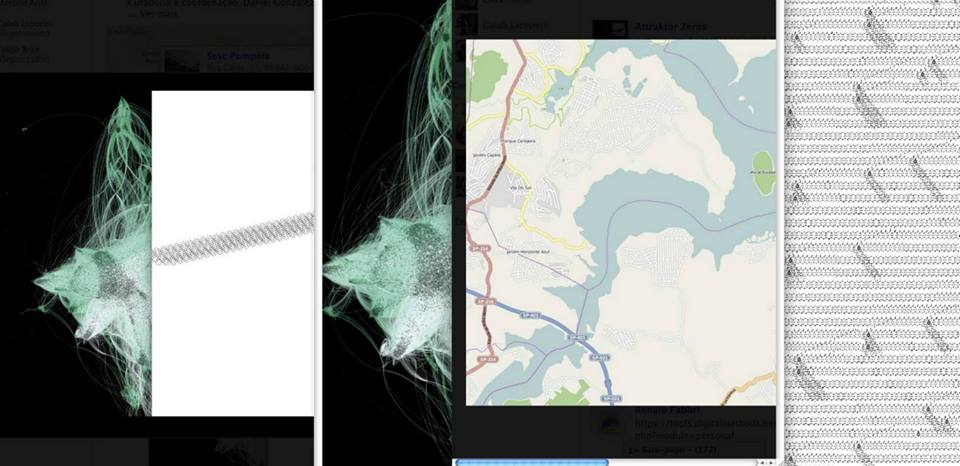
\includegraphics[scale=.45]{figs/ppr}
\caption{An example artistic image by Pedro Paulo Rocha and derived from our network visualizations.
	For further information please see Section~\ref{sec:ppr}}
\label{fig:ppr}
\begin{flushleft}\footnotesize
Source: Provided by the artist Pedro Paulo Rocha. Image derived from other images by the author.\
\end{flushleft}
\end{center}
\end{figure}

\section{Mega networks: connecting many Facebook ego networks}\label{sec:megarrede}
The most usual social networking platform nowadays is Facebook.
In this platform, one cannot have more than 5000 friends.
To analyze larger friendship network social structure through Facebook,
we started merging the networks from distinct users.
From this procedure we obtained networks with tenths of thousands of participants
and even a few which reached the scale of hundreds of thousands.
Such practice started at AVLAB 6 in SESC Pompéia (directed by Daniel Gonzales Xavier)
and was further developed in a number of occasions by us and other researchers.
Figure~\ref{fig:megarrede} exemplifies one of such structures.
\begin{figure}[h!]
\begin{center}
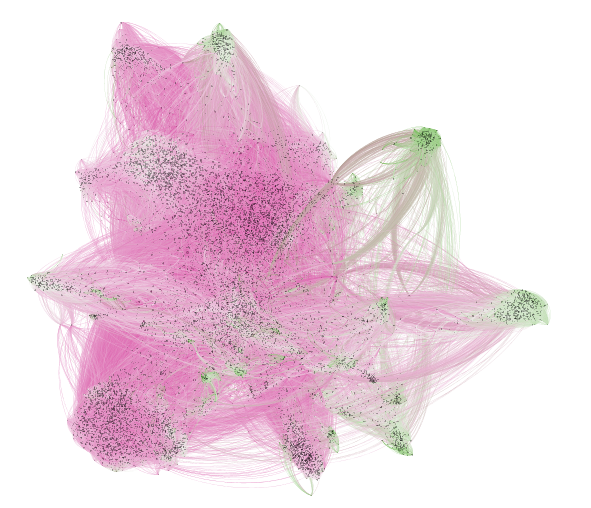
\includegraphics[scale=.45]{figs/megarrede}
\caption{An example visualization of a mega network with tenths of thousands of participants derived from Facebook ego networks.
	For further information please see Section~\ref{sec:megarrede}}
\label{fig:megarrede}
\begin{flushleft}\footnotesize
Source: By the author.\
\end{flushleft}
\end{center}
\end{figure}
% arte pelo Pedro Paulo Rocha

\section{Social structures live streaming (networks and language-related)}\label{sec:sss}
A strong trait I could observe with the cycles of information gathering and diffusion (see Section~\ref{sec:colDif})
is the timid appropriation of the social structures by their participants.
Some people are enchanted by the figures,
others by the concepts and by the perception of the social aspect of themselves,
sometimes called ``network being'' or `` I-network '' by interested parties during the broadcasts.
In these contexts, academic theories, such as the Network Actor Theory (Latour),
were rarely recalled directly, even by specialists.
The efficiency of the intuitive discourse to communicate about these interests is impressive.
The impulse to report the impressions resembles the urge to report dreams,
with glimpses of subtle and unconscious structures and sequential forgetfulness.
In this context, in order to spread about how our traces can be observed and taken advantage of,
we programmed screens of social structures streaming in HTML pages.
Only Twitter was used, and networks yield by retweets,vocabulary and hashtags were contemplated.
The screen could also display recent tweets, more occurring words, co-occurrences,
and other simple text information.
These screens were used e.g. in the Arena NET Mundial event
and in mobilizations such as the one identified with the \#ocupaGOV hashtag.
Figures~\ref{fig:telao1} and~\ref{fig:telao2} exemplify such interfaces.
They were updated live as tweets were sent by all Twitter users whose messages
contained the selected hashtags.
The source code is publicly available in~\cite{teloes}.

\begin{figure}[H]
  \centering
    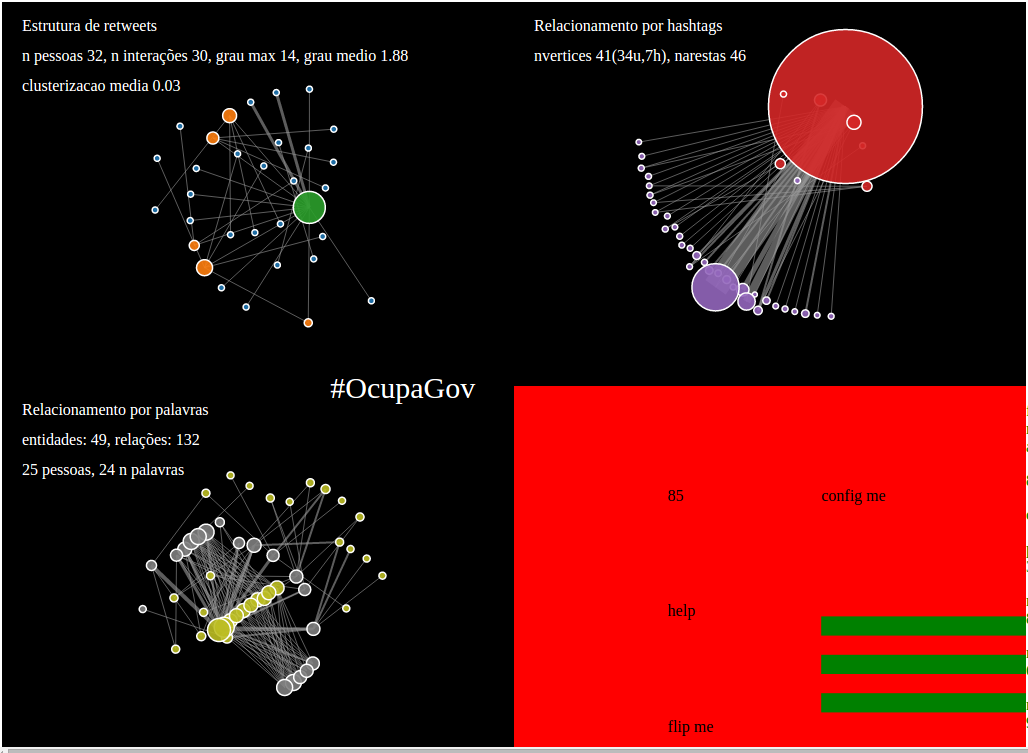
\includegraphics[width=.85\textwidth]{figs/telao1.png}
  \caption{Network interfaces of the live social structures streaming gadgets we programmed.
	Further information is on Section~\ref{sec:sss}.}\label{fig:telao1}
\begin{flushleft}\footnotesize
Source: By the author.\
\end{flushleft}
\end{figure}

\begin{figure}[H]
  \centering
    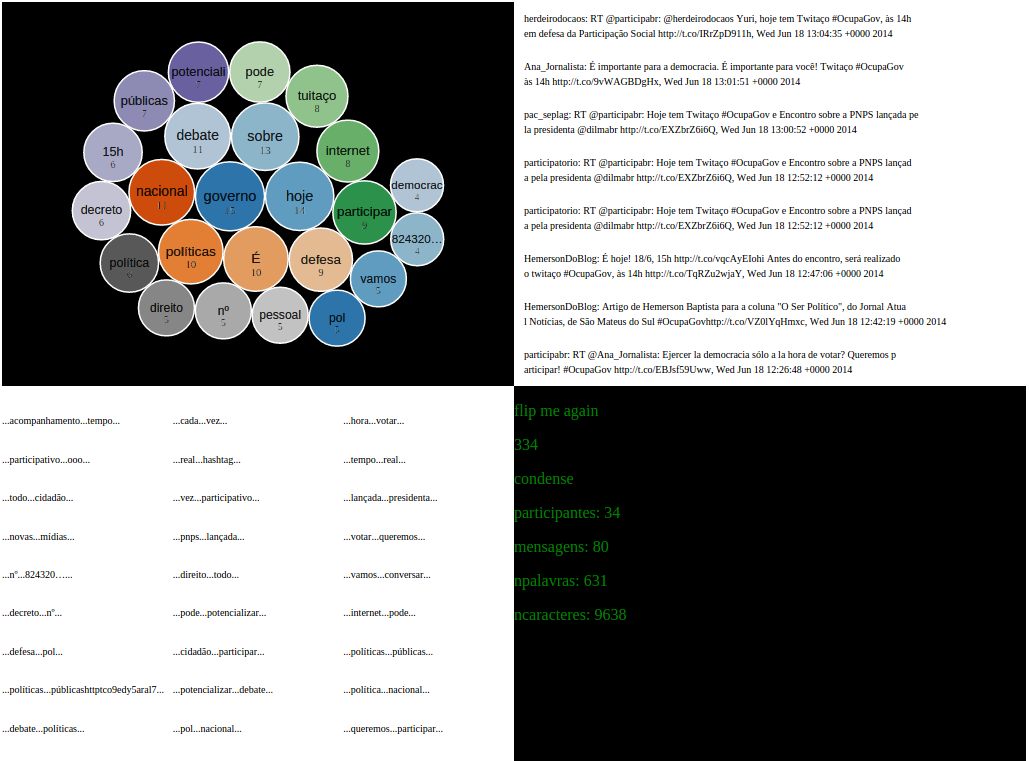
\includegraphics[width=.85\textwidth]{figs/telao2.png}
  \caption{Language-related interfaces of the live social structures streaming gadgets we programmed.
	Further information is on Section~\ref{sec:sss}.}\label{fig:telao2}
\begin{flushleft}\footnotesize
Source: By the author.\
\end{flushleft}
\end{figure}

\section{Ubiquity of inequality: a simple model that explains why power laws are so frequently found in empirical data}
	Inequality has always been a crucial issue for human kind, particularly concerning the highly unequal distribution of wealth, which is at the root of major problems facing humanity, including extreme poverty and wars.
	A quantitative observation of inequality has become commonplace in recent years
	with the expanding recognition that many natural and man-made systems can be represented as scale-free networks,
	whose distribution of connectivity obeys a power law.
	These networks may be generated by the preferential attachment for the nodes, within the so-called rich-gets-richer paradigm.
	In~\cite{ubiIne} we introduce a simple model that explains the ubiquity of inequality, based on three simple assumptions applied to a generic system with numerous parts.
	The first assumption is the diversity of the components.
	The second assumption is a uniform distribution of resources for individual components.
	The third assumption is that the amount of each resource input to the system is fixed.
	This implies that the more resources are allocated per component, the less numerous are such components,
	with the conservation of the amount of resources distributed through $component\; wealth = \frac{resources}{component}$.
	The second and third assumptions are conservation laws: energy is conserved through each resource and through component wealth.
	This can be geometrically described by the distribution of object sizes in an n-dimensional Euclidean space.
	Applying these assumptions to a generic system results in a power-law distribution, whose coefficient is the number of inputs that are independent from each other,
	i.e. the dimensionality of the allocated resources.
	Even though there is no restriction to the value of the coefficient,
	in practice we observe that existing systems normally exhibit a coefficient between 1.5 and 3.0.
	With our simple model it is not possible to determine whether this limitation in the coefficient values arises from a fundamental principle, but we indicate reasonable hypotheses.
	The assumptions in the model lead to a framework analogous to the laws of thermodynamics:
	conservation of resources and a time arrow pointing to inequality.
	Since these assumptions are easily justified based on established knowledge,
	the model proves unequivocally that inequality is ubiquitous.
	We also discuss ways to control this tendency to inequality,
	which is analogous to a decrease in entropy in a closed system induced by an external action.

\section{Systematic measurements related to the two-sample Kolmogorov-Smirnov test}
The two-sample Kolmogorov-Smirnov test relate the number of samples and the Kolmogorov-Smirnov statistic
to a confidence level in rejecting the null hypothesis (that the underlying distributions of the samples are the same).
However, if sample sizes are large enough, the test rejects the null hypothesis even with arbitrarily small differences
in the distributions.
In terms of Section~\ref{sec:ks}, $c'$ can be arbitrarily large for any non-zero value of
$D_{n,n'}=sup_x[F_{1,n}-F_{2,n'}]$
if the sample sizes $n$ and $n'$ are large enough.
As a way to better grasp these relations between 
$c'$,
$D_{n,n'}=sup_x[F_{1,n}-F_{2,n'}]$,
$n$ and $n'$, we made systematic measurements using many distributions
(normal, uniform, Weibull, power) and different parametrizations.
These measurements are presented in~\cite{kolmSmir}.

\section{The Algorithmic Autoregulation (AA) software development methodology}\label{sec:aa}
In~\cite{aaPaper} we present a new self-regulating methodology for coordinating distributed team work called Algorithmic Autoregulation (AA),
based on recent social networking concepts and individual merit.
Team members take on an egalitarian role, and stay voluntarily logged into so-called AA sessions for part of their time 
(e.g. 2 hours per day), during which they create periodical logs - short text sentences - 
they wish to share about their activity with the team.
These logs are publicly aggregated in a website and are peer-validated after the end of a session,
as in code review. 
A short screencast is ideally recorded at the end of each session to make AA logs more understandable.
This methodology has shown to be well-suited for increasing the efficiency of distributed teams working on 
Global Software Development (GSD), as observed in our reported experience in actual real-world situations.
This efficiency boost is mainly achieved through 1) built-in asynchronous on-demand communication in 
conjunction with documentation of work, products, and processes, and 2) reduced need for central management,
meetings or time-consuming reports.
Hence, the AA methodology legitimizes and facilitates the activities of a distributed software team.
It thus enables other entities to have a solid means to fund these activities, 
allowing for new and concrete business models to emerge for very distributed software development. 
AA has been proposed, at its core, as a way of sustaining self-replicating hacker initiatives.
These claims are discussed in a real case-study of running a distributed free software hacker team called Lab Macambira.
This work was important for maturing concepts related to social networks and thus contributed to the presented thesis.

\section{Social participation (OWL) ontologies}
As a way to integrate participatory mechanisms, some OWL ontologies were developed within our research.

\subsection{OPS: the Social Participation (OWL) Ontology}
Participatory democracy advances in virtually all governments and especially in South America which presents a mixed culture and social predisposition.
 In 2012, civil, academic and governmental parties started elaborating the ``Social Participation Common Vocabulary'' (\vcps\ from the Brazilian name \emph{Vocabul\'ario Comum de Participa\c{c}\~ao Social}), as a public and online process. By May 2013, first reference documents were publicized, together with preliminary \owl\ code, logos, and a diagram for a general ``public consultation''.
The \corais\ platform kept online records of the process, like discussions and text drafts. 
The article~\cite{ops} presents this material and proposes, based on it, the ``Social Participation Ontology'' (\ops\ from the Brazilian name \emph{Ontologia de Participa\c{c}\~ao Social}). To create  this new ontology, these steps were followed: correction of ontological contradictions and \owl\ errors in \vcps; inclusion of concepts documented in the \corais\ platform (but not present in \vcps) in a preliminary version of \ops; entity name standardization; translation of labels to Portuguese, Spanish and English; an ontology expansion; creation of linked data examples and  a \sparql\ endpoint; compilation of use cases from researchers and public managers. Ongoing work involves further adoption of \ops\ by the official Brazilian federal portal for social participation and  NGOs, and linkage to other ontologies for participation. The \ops\ is being used as an upper ontology, and all classes linked further to \foaf\ and \bfo\ as higher upper ontologies.

\subsection{OPa: the ParticipaBR federal social participation web portal (OWL) Ontology}\label{sec:opa}
There were two very distinct ontologies for the ParticipaBR Brazilian federal social participation web portal.
The first ontology, centered around the concepts of Portal, Participant, Community and Participation Mechanism,
was conceptualized by the community by idealizations of what a
federal social participation portal should be and the main documentation is available in~\cite{opa0}.
The second ontology was derived from the data of the portal and is available in~\cite{opa}.
The first ontology was interesting for the specialists and might help in creating new web portals but did not fit
ParticipaBR data: ontology classes and properties did not find correspondent entries while
ParticipaBR items did not have correspondent structures in the ontology.
Therefore the second ontology was created.

\subsection{OntologiAA: the AA (OWL) Ontology}\label{sec:ontologiaa}
An ontology for the AA mechanism described in Section~\ref{sec:aa} was developed and is documented in~\cite{opa}.
This ontology is depicted in Figure~\ref{fig:aaOn}.
\begin{figure}[h!]
\begin{center}
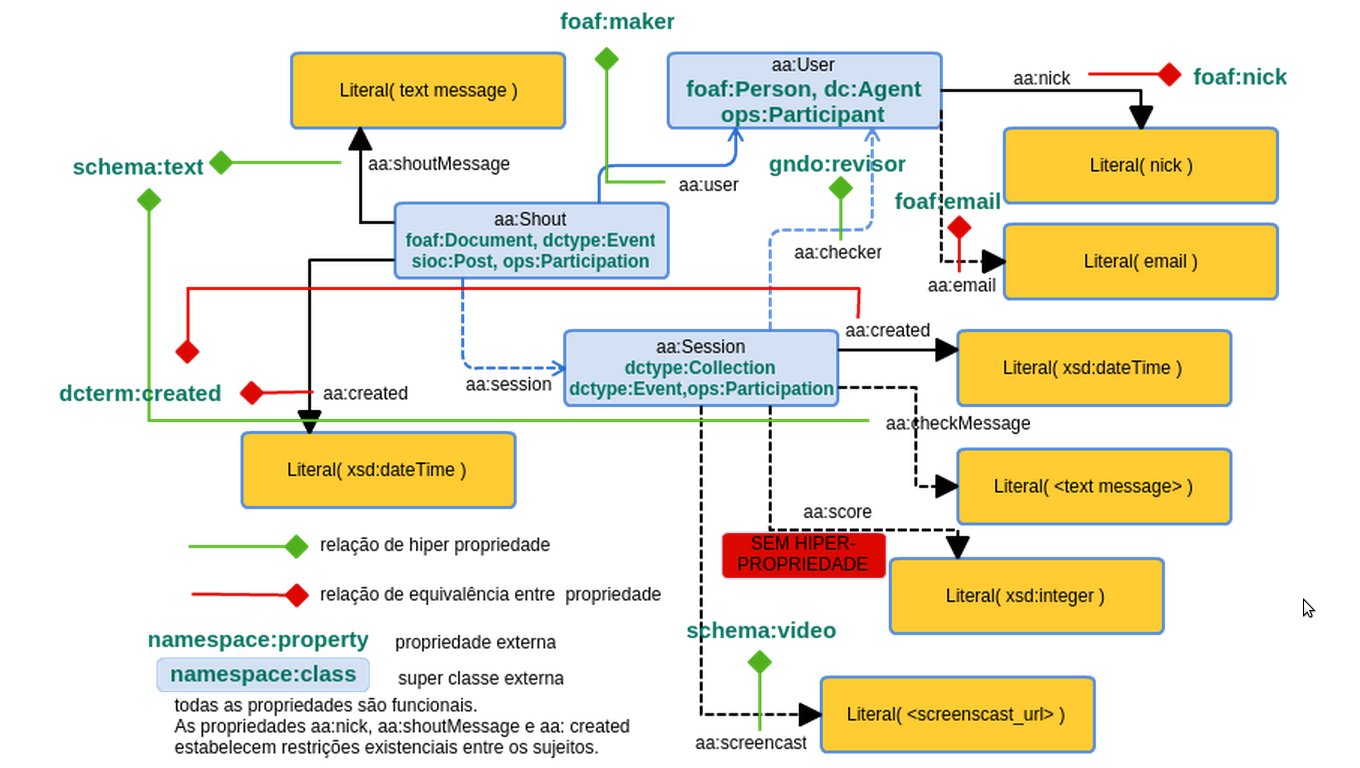
\includegraphics[scale=.3]{figs/ontologiaa}
\caption{A pictorial representation of the AA Ontology.
	For further information please see Section~\ref{sec:ontologiaa}}
\label{fig:aaOn}
\begin{flushleft}\footnotesize
Source: By the author.\
\end{flushleft}
\end{center}
\end{figure}
\subsection{OCD: Cidade Democrática (OWL) Ontology}
An ontology for the Cidade Democrática civil social participation platform was developed and is documented in~\cite{opa}.
For this ontology we developed the data driven ontology synthesis method presented in Section~\ref{sec:ontSyn}
and that was used for obtaining the second ontology described in Section~\ref{sec:opa}.

\subsection{Social Library: conference, forum, council, ombudsman, public consultation, dialogue table, decree 8.243 and IPEA}
The OBS (Social Library Ontology, from the Portuguese ``Ontologia da Biblioteca Social)
and the VBS (Social Library Vocabulary, from the Portuguese ``Vocabulário da Biblioteca Social)
was derived from two types of sources: specialists (political authorities)
and the decree 8.243 that organized the Brazilian social participation instances.
The specialists contributed in two manners: by means of a Workshop given by the author 
of this thesis in the Presidency Palace in Oct/20/2014
and by means of dedicated interviews.
Social participation instances and mechanisms were systematized and general
social participation conceptualizations given separately by the Brazilian Presidency
and the IPEA (Institute for Applied Economic Research).
Core documentation is in~\cite{opa}.

% Conselhos, Foruns, Mesas Redondas, etc. Casos feitos com especialistas, casos feitos a partir de documentações
\section{Genesis of this work: complex social networks analysis by emails}
The first written systematization of our findings among networks derived from email lists
is~\cite{comp1}.
It was important for a several reasons: we confirmed the scale-free outline of the connectivity distribution
in these networks;
we first observed the asymmetry of edges;
the article invoked disrupting discussion in email lists and private messaging.
This work received collaborations of Vilson Vieira da Silva Junior, Lucas da Silva Oliveira
and Prof. Dr. Ricardo Fabbri
and was presented in the XVI Meeting for Computational Modeling.
% in metareciclagem
% presented by ricardo fabbri
\section{United Nations Development Program consulting}\label{sec:undp}
In the year of 2014 this research was endorsed by the United Nations Development program
with a consulting contract (2013/00056, project BRA/12/018).
The collaboration was centered around complex networks,
natural language processing/text mining, linked data and social participation,
all of which are approached in Chapter~\ref{ch:int}.

\subsection{Partnership with the Brazilian Presidency}
This consulting was proposed as a partnership between me
and the Brazilian Presidency.
Many of our meetings and immersions were held by the Brazilian Palace (\emph{Palácio do Planalto})
and I could learn deeply by working with specialists and authorities.
The supervisor was Ricardo Poppi who was then the presidential general coordinator of new media.
More names of people involved in this collaboration are on the Acknowledgments in the beginning of this thesis.

\subsection{Description of each product}
\begin{itemize}
	\item Product 1: the first ParticipaBR ontology~\cite{opa0}.
	\item Product 2: context, triplification of data, example of usage~\cite{pnud2}.
	\item Product 3: resources classification and recommendation~\cite{pnud3}.
	\item Product 4: proposals of enhancements for the ParticipaBR portal~\cite{pnud4}.
	\item Product 5: integration of ParticipaBR and other participation instances~\cite{opa}.
\end{itemize}

\section{Govern art}\label{sec:govArt}
Many of the developments presented in this thesis were accompanied by the construction of online gadgets
and some of them were artistic.
As we labored with government parties and issues,
the concept of ``government art'' emerged.
The proposal is to make art with government/State symbols.
Some of the realized examples of govern art are in~\cite{aars}.
The Meteor company unfortunately stopped their free services which
allowed these gadgets to keep functioning online.

\section{Sounding Skull: a Rilke proposed transcendental experiment}\label{sec:soundSkull}
Rainer Maria Rilke proposed transdisciplinary experiments by trying to hear the
sounds of the grooves in the cranium~\cite{rilke}.
We created a performance group to make such experiments.
This was important for our research as an interface
by means of which different backgrounds could be exchanged by the participants.
The performers of the Sounding Skull group are:
Prof. Dr. Massimo Canevacci, Prof. Dr. Marília Pisani,
Rita Wu, Caleb Mascarenhas Luporini and Renato Fabbri.
There were also occasional but important participation
by Juliana de Souza and Gulherme Lunhani.
Most important presentations were in the AVLAB 6 (an event about art, media and politics)
and in closing the International Critical Theory Conference of Rome (online participation).

\section{Ideal ideas: a physical modeling of the mind}
Thought can be conceived as constituted by ideas.
Ideas can be conceived in a way that any set of ideas is an idea.
In~\cite{idealIdeas} we present a physical and formal description of the
thought in such conceptualization.

\section{Webpages}
% ARS, texto para pedro, MMISSA, MyNSA
There were many webpages produced by this research.
Maybe the most important of them are the ones directly related
to Social Network Analysis and the endeavors for collection and diffusion of information~\cite{sfARS,rfARS}.
One interesting instance is the online publication of the text ``Cognitive clouds and the unification of humanity''~\cite{nuvens}
by the Cyberium transmedia collective and the Nós Digitais digital cultural pole.
Some pages are not online anymore, such as the ones referred to in Section~\ref{sec:govArt},
mainly because free services were withdrawn.
All texts and software developed in this research are available in online pages,
mainly hosted by Github and arXiv but also in Wikis and Sourceforge.
A simple but useful example of a gadget used by means of a webpage that
stood the test of time is an AA interface~\cite{aaclient} for displaying the shouts
(see Section~\ref{sec:aa}).

\section{Collection and diffusion of information in social networks}\label{sec:colDif}
In realizing the proposal of this research of enabling the participants to take action
in their networks by means of scientific knowledge, it was considered central
to tackle the collection and diffusion of information.
This was achieved in a number of ways which are documented in this thesis and bibliography items.
We next expose four main practices we developed which are not documented elsewhere.

\subsection{Progressive network activation from peripherals to hubs for a crowdfunding}
This is maybe the most powerful mechanism by which we performed collection and diffusion of information.
The results were very effective in spreading information about social networks,
in gathering knowledge from diverse parties and in modifying the social structures
in which I participate.
Most concretely, academics came to São Carlos for formal meetings,
new collaborations were established (such as the UNDP consultation described in Section~\ref{sec:undp}),
money was obtained (various contributors transferred a total of about 3000 Brazilian reais)
and my Facebook network increased about 50\% with individuals interested in the research.
The process consisted in:
\begin{enumerate}
	\item Downloading my Facebook friendship Network. This was done by means of the Netvizz software,
		which is not possible nowadays and requires scrapping of Facebook pages because of new license issues.
	\item Sorting my friends from the less connected to the more connected, i.e. from my friends that have less friends in common with me to the ones that have more friends in common; i.e. from periphery to hubs.
	\item Sending private messages for each of my friends, in such order.
		The messages were derived from a template I conceived in which I exposed the research and information diffusion process.
	\item Making steps 1-3 for three times.
\end{enumerate}
In each cycle of steps 1-3, my friendship network grew about 15\% and there were typical reactions in each cycle.
In the first cycle, my Facebook contacts reacted with estrangement and replies such as ``what are these network structures?'',
``what are you doing? I can't understand!'', ``I never though of such a thing as these networks''.
In the second cycle, they replied with interest and support.
In the third cycle, they were establishing collaborations with visits, elaboration of documents and technologies and
co-working proposals.

The main problem of these results is that they were not still confirmed by performing the experiment again.
Even so, the data can be organized by downloading the personal data in the Facebook interface.
Given that the diffusion process was done in Dec/2012-Jan/2013, it was frequently thought of by fellow specialists as
having some influence in the civil society mobilization that occurred in Brazil in Mar/2013 and thereafter.
A very simple PDF document was built afterwards for delivering back these results to the networks~\cite{docDif}.

\subsection{Instantaneous network activation by betweenness and closeness centralities}
This was first thought by meetings with the artist and activist Pedro Paulo Rocha.
The idea was to activate the network not by means of a longstanding process such
as described in the last section, but by an ephemeral endeavor.
There were some artistic performances with this proposal, in which I did
not participate.
Notwithstanding, there was one of these instantaneous activation processes that
I have done in conjunction with other specialists which was rather interesting.
In analyzing Facebook ego friendship networks, the set of $\approx 50$ members with
the greatest betweenness centrality was disjoint with the set of $\approx 50$ members
with the greatest closeness centrality, which is very unexpected.
Therefore I proposed that one should send the same message to both set of friends separately.
The messages were different for each person performing the experiment,
and it was also about something they were interested about and wanted to spread and get feedback.
The result was systematic: the set of friends with greatest betweenness always reacted very friendly
with encouraging messages and sharing the original message in their timelines.
The set of friends with greatest closeness always reacted with many leaving the chat group
and with no replies.
We hypothesize that these reactions are because the large betweenness set of friends is more
likely to have control over the information flowing in the corresponding ego network while
the large closeness set of friends is more likely to observe/receive influenced by the information.

This experiment was performed by partners related to the consulting reported in Section~\ref{sec:undp}
and other partners involved in making an international technoshamanic festival.

\subsection{Massive tagging in Facebook and email crossposting}
One very simple process by which we performed collection and diffusion of information
was by tagging many friends in Facebook posts.
Currently, one can tag up to 99 friends in a post
and we did not find any limit for tagging friends in comments.
If one makes abusive use of tagging (too many posts or too many comments)
the Facebook platform sometimes restricts the permissions of that user.
Even so, I have made many posts with up to 99 friends tagged and tagged more
friends in the comments and made experiments such as the ones described in the
last sections and never got restricted.
It seems that the platform has some automated behavior but employees actually
perform the restrictions at least in some cases.
These employees might check the posts, tagging and messages to see if it is
really spam or in anyway abusive.

Another powerful way by which I many times performed diffusion and collection
of information is by crossposting, i.e. by sending a message to many email lists
at the same time.
I find this very effective but the email list users often report such practice
as abusive.
Even so, no one has ever sent me a message reporting discomfort with my crossposts.
There was one occasion some years ago when a user replied with a challenge for
arguing why the crosspost what appropriate and then made some good contributions.
I personally perceive that this prejudice against crosspost is one of the main reasons
why email groups are losing users to other communication protocols such as Facebook, Whatsapp, Telegram and Diaspora.

\subsection{SERVDDCR online video conferences}

\section{Anthropological physics}
The study of complex systems can be undertaken as a physics endeavor,
specially if complex networks and statistics are into play. When the complex
system is constituted by people, intriguing questions arise from diverse field such as math, ethics, and sociology. The “anthropological physics”is an approach to these scenarios that enables scientific research while resolving ethical and moral issues by an open study of the self.
	It yields a transdisciplinary practice whose relevance emanate from anthropological
and physical matters, from human constituted systems and natural laws.
A sweet spot was found in recent civil, government and academic efforts~\cite{opa,ensaio}, and has been called anthropological physics. General characteristics are:
\begin{itemize}
	\item Exposure of the researcher to the environment of interest, such as virtual social networks.
	\item Use of the annotations from the exposure, be them activity logs, friendship or interaction networks, textual contents, etc.
	\item Upon need, expansion of observations to encompass open datasets or data donated by partners.
	\item Observance of natural laws as they appear in network structures and natural language.
	\item All resources are kept as open and publicized as possible, including software, data, and writings.
\end{itemize}                                                                                                                                     
A short report the first insights regarding anthropological physics is on~\cite{anPhy}.
 
% conceitualização básica, artigo e conferências
\section{Listing of documents written, videos recorded, conferences attended and artistic presentations}
% https://www.dropbox.com/home/Public/presidencia
% https://dl.dropboxusercontent.com/u/22209842/presidencia/SistemaMonitoramentoPBR.pdf
% rcpln
% artigos
% conferências: duas nexos+ccdc+linguística+sifiscs+ufpa+
% apresentações na SGPR, imersões, arenaNETmundial
% Labicbr, Mirosc
% vivace

\end{apendicesenv}
